\documentclass[conference]{IEEEtran}
\IEEEoverridecommandlockouts

\usepackage{cite}
\usepackage{amsmath,amssymb,amsfonts}
\usepackage{algorithmic}
\usepackage{graphicx}
\usepackage{textcomp}
\usepackage{xcolor}
\usepackage{booktabs}
\usepackage{array}
\usepackage{url}
\usepackage{tikz}
\usetikzlibrary{arrows.meta,positioning,fit,calc}

\def\BibTeX{{\rm B\kern-.05em{\sc i\kern-.025em b}\kern-.08em
    T\kern-.1667em\lower.7ex\hbox{E}\kern-.125em X}}

% ---- Placeholder macro: every unresolved project value is shown in red ----
\newcommand{\ph}[1]{\textbf{\textcolor{red}{[#1]}}}

% ---- TikZ styles for the architecture figures ----
\tikzset{
  b/.style={draw,rounded corners=1pt,align=center,font=\scriptsize,
            text width=2.4cm,minimum height=0.55cm,inner sep=2pt},
  m/.style={b,fill=blue!12,thick},
  d/.style={b,fill=gray!10},
  ar/.style={-{Stealth[length=1.6mm]}}
}

\begin{document}

\title{Smart Literature Review Assistant using\\
VectorRAG, GraphRAG and HybridRAG}

\author{
\IEEEauthorblockN{Samudrala Sai Mrudhula}
\IEEEauthorblockA{
Dept. of Artificial Intelligence and Data Engineering\\
Malaviya National Institute of Technology\\
Jaipur, India\\
2023UAI1798
}
\\[1em]
\IEEEauthorblockN{Deepshikha Raj}
\IEEEauthorblockA{
Dept. of Artificial Intelligence and Data Engineering\\
Malaviya National Institute of Technology\\
Jaipur, India\\
2023UAI1803
}
}

\maketitle

\makeatletter
\renewenvironment{abstract}{%
    \begin{center}
        \bfseries Abstract
    \end{center}
    \vspace{-0.5em}
    \normalfont\small
}{%
    \par
}
\makeatother

\begin{abstract}
The rapid growth of scientific publications makes it increasingly difficult for researchers to efficiently locate and synthesize relevant information from research papers. Large language models (LLMs) can support literature question answering, but they may generate fluent responses that are unsupported by the source documents. Retrieval-Augmented Generation (RAG) addresses this limitation by grounding generated responses in retrieved evidence; however, the choice of retrieval strategy can significantly affect retrieval relevance and answer faithfulness. This paper presents a Smart Literature Review Assistant that implements and evaluates three retrieval strategies, namely VectorRAG, GraphRAG, and HybridRAG, in an end-to-end pipeline for scientific literature question answering. The study is based on a recent evaluation of vector-based, graph-based, and hybrid RAG systems for scientific literature chatbots, which uses text-embedding-ada-002 for embedding and gpt-4o-mini for generation. In contrast, our implementation adopts a resource-efficient open-source configuration using sentence-transformers/all-MiniLM-L6-v2 for semantic representation and google/flan-t5-small for answer generation. The three retrieval strategies are evaluated in two scenarios: question answering over a single uploaded research paper and retrieval from a multi-paper database. Performance is assessed using cosine similarity and faithfulness, and the obtained results are compared with those reported in the reference study. The results show that HybridRAG achieves the highest overall performance under the lightweight configuration, obtaining a cosine similarity of 0.614 and faithfulness of 0.771 in the single-paper setting, while achieving 0.581 cosine similarity and 0.741 faithfulness in the multi-paper setting. VectorRAG follows with 0.592 cosine similarity and 0.752 faithfulness for single-paper retrieval, whereas GraphRAG achieves 0.558 and 0.708, respectively. The comparison highlights the practical differences among VectorRAG, GraphRAG, and HybridRAG under a lightweight open-source configuration and demonstrates the trade-offs between retrieval relevance, answer grounding, and computational efficiency.
\end{abstract}

\begin{IEEEkeywords}
Retrieval-Augmented Generation, VectorRAG, GraphRAG, Hybrid Retrieval,
Scientific Literature Question Answering, Semantic Retrieval, Faithfulness
\end{IEEEkeywords}


%=====================================================================
\section{Introduction}
The number of scientific publications continues to grow, which makes literature exploration increasingly time-consuming. Traditional keyword-based retrieval depends on lexical overlap between a query and a document and can miss relevant work expressed with different terminology \cite{robertson2009bm25}. Neural embedding models address part of this limitation by mapping text into dense vectors in which semantic proximity can be measured \cite{reimers2019sbert,karpukhin2020dpr}. Large language models (LLMs) built on the Transformer architecture \cite{vaswani2017attention} can additionally synthesize answers in natural language, but they may generate statements that are not supported by any source, a failure mode commonly called hallucination \cite{ji2023hallucination}.

Retrieval-augmented generation (RAG) conditions a generator on passages retrieved from an external corpus, which can ground answers in identifiable evidence \cite{lewis2020rag,gao2023ragsurvey}. In scientific literature question answering, the quality of the answer depends strongly on which evidence is retrieved. Vector retrieval selects text that is semantically similar to the query, whereas graph-based retrieval exploits explicit entities and relationships and can support multi-hop information needs \cite{edge2024graphrag,peng2024graphragsurvey}. Hybrid approaches combine both signals \cite{sarmah2024hybridrag}. This progression from VectorRAG to GraphRAG to HybridRAG motivates a systematic comparison of retrieval strategies for scientific papers.

Ghanadian et al.\ \cite{ghanadian2026base} evaluated vector-based, graph-based and hybrid RAG for scientific literature chatbots in a single-paper and a multi-paper scenario. Their configuration relies on \texttt{text-embedding-ada-002} and GPT-4o-mini, which are proprietary and accessed through an external service. This paper asks a related practical question: \emph{how do vector-based, graph-based and hybrid retrieval strategies affect the quality and grounding of scientific literature question answering when implemented with a lightweight open-source embedding and generation configuration?}

The contributions of this work are as follows.
\begin{enumerate}
\item An end-to-end literature question-answering assistant that accepts research papers and returns answers with references to their supporting evidence.
\item An implementation of VectorRAG, GraphRAG and HybridRAG using \texttt{all-MiniLM-L6-v2} and \texttt{flan-t5-small}, as a lightweight open-source alternative to the configuration of \cite{ghanadian2026base}.
\item An experimental comparison of the three strategies in single-paper and multi-paper scenarios using cosine similarity and faithfulness.
\item An analysis of how our results relate to those of the base paper, with explicit discussion of the differences between the two experimental setups.
\item A discussion of source traceability and observability for literature assistants, stating which capabilities are implemented.
\end{enumerate}
This work does not propose a new RAG or graph algorithm. Its contribution is an implementation and evaluation study.

%=====================================================================
\section{Related Work}
\subsection{Traditional Information Retrieval}
Classical retrieval represents documents and queries as sparse term vectors \cite{salton1975vsm} and ranks them with weighting schemes such as BM25 \cite{robertson2009bm25}. These methods are efficient and transparent but are limited by vocabulary mismatch between query and document.

\subsection{Neural Semantic Retrieval}
Dense representations map text to a continuous space where related passages are close. Word embeddings \cite{mikolov2013word2vec} and pretrained Transformers \cite{devlin2019bert} led to sentence-level encoders such as Sentence-BERT \cite{reimers2019sbert} and to dense passage retrieval \cite{karpukhin2020dpr}. MiniLM compresses larger Transformers into small models through self-attention distillation \cite{wang2020minilm}, and the \texttt{all-MiniLM-L6-v2} model is distributed through the Sentence-Transformers library \cite{hf_minilm}.

\subsection{Retrieval-Augmented Generation}
Lewis et al.\ \cite{lewis2020rag} combined a retriever with a sequence-to-sequence generator for knowledge-intensive tasks. Later surveys describe the evolution of RAG pipelines and their evaluation challenges \cite{gao2023ragsurvey}. Evaluation frameworks such as RAGAS assess faithfulness and relevance without requiring reference annotations for every dimension \cite{es2024ragas}.

\subsection{VectorRAG}
VectorRAG indexes chunk embeddings and retrieves the chunks most similar to the query embedding, typically with an approximate or exact nearest-neighbor index \cite{johnson2021faiss}. It is simple and effective for semantic matching, but it treats chunks independently and does not model explicit relations between them.

\subsection{GraphRAG}
GraphRAG organizes information as entities and relations. Edge et al.\ \cite{edge2024graphrag} construct an entity graph from a corpus, detect communities and use community summaries to answer corpus-level questions. A survey of graph-based RAG reviews graph construction, retrieval and generation strategies \cite{peng2024graphragsurvey}. In this paper GraphRAG refers to relationship-aware retrieval in this general sense; the specific graph construction used here is described in Section~\ref{sec:graph}.

\subsection{Hybrid RAG}
HybridRAG combines knowledge-graph and vector retrieval so that semantic and relational evidence can complement each other. Sarmah et al.\ \cite{sarmah2024hybridrag} report this combination for question answering over financial documents.

\subsection{Scientific Literature Assistants}
PaperQA is an LLM-based agent for answering questions from scientific papers \cite{lala2023paperqa}. The study of Ghanadian et al.\ \cite{ghanadian2026base} is the central reference of this paper because it directly compares VectorRAG, GraphRAG and HybridRAG for scientific literature chatbots. Table~\ref{tab:related} summarizes the related work discussed above.

\begin{table}[t]
\caption{Summary of Related Work}
\label{tab:related}
\centering
\footnotesize
\begin{tabular}{p{1.35cm}p{1.45cm}p{1.35cm}p{2.5cm}}
\toprule
Work & Retrieval & Domain & Scope note \\
\midrule
Lewis et al.\ \cite{lewis2020rag} & Dense passage & Open-domain & Introduces the RAG paradigm \\
Edge et al.\ \cite{edge2024graphrag} & Entity graph, communities & Private text corpora & Targets corpus-level (global) questions \\
Sarmah et al.\ \cite{sarmah2024hybridrag} & Knowledge graph + vector & Financial documents & Domain-specific evaluation \\
Lála et al.\ \cite{lala2023paperqa} & Agent-based retrieval & Scientific papers & LLM-agent design \\
Ghanadian et al.\ \cite{ghanadian2026base} & Vector, graph, hybrid & Scientific literature & Proprietary embedding/generation models \\
\bottomrule
\end{tabular}
\end{table}

%=====================================================================
\section{Base Paper and Research Gap}
\label{sec:base}

\subsection{Base Paper}

Ghanadian et al.~\cite{ghanadian2026base} propose a scientific literature chatbot based on Retrieval-Augmented Generation (RAG) that combines vector-based and graph-based retrieval to answer questions from scientific literature. The study compares three retrieval approaches: VectorRAG, GraphRAG, and Hybrid RAG. The evaluation considers two use-case scenarios: (i) retrieval from a single uploaded research paper and (ii) retrieval from a multi-paper database.

For evaluation, the authors construct synthetic test sets using GPT-4o-mini and subsequently assess the quality of the generated questions, answers, and contexts using human annotation. The single-paper test set contains 500 question--answer--context instances, while the multi-paper test set contains 60 instances. The annotation evaluates whether the retrieved context is related to the question and whether the generated answer fully addresses the question. The reported context relevance is 94.2\% for the single-paper test set and 81.6\% for the multi-paper test set, while answer completeness is 92\% and 85\%, respectively. \cite{ghanadian2026base}

The main RAG evaluation uses two metrics: \textit{cosine similarity} and \textit{faithfulness}. Cosine similarity measures the semantic similarity between the generated response and the corresponding ground-truth answer, whereas faithfulness measures whether the generated response is supported by the retrieved context. Higher values indicate greater semantic similarity and stronger grounding, respectively. \cite{ghanadian2026base}

The base paper reports the performance of VectorRAG, GraphRAG, and Hybrid RAG for both evaluation scenarios, as summarized in Table~\ref{tab:baseresults}. The reported results show that Hybrid RAG achieves the highest mean cosine similarity and faithfulness in both the single-paper and multi-paper settings. These results provide the primary reference point for evaluating the performance of the proposed system.

\begin{table}[t]
\centering
\caption{Performance reported by the base paper.}
\label{tab:baseresults}
\begin{tabular}{lcccc}
\hline
\textbf{Method} &
\multicolumn{2}{c}{\textbf{Single Paper}} &
\multicolumn{2}{c}{\textbf{Multi-Paper}} \\
& Cosine & Faithfulness & Cosine & Faithfulness \\
\hline
VectorRAG &
0.670 $\pm$ 0.189 &
0.841 $\pm$ 0.137 &
0.651 $\pm$ 0.188 &
0.830 $\pm$ 0.133 \\
GraphRAG &
0.654 $\pm$ 0.184 &
0.785 $\pm$ 0.153 &
0.633 $\pm$ 0.174 &
0.761 $\pm$ 0.149 \\
Hybrid RAG &
\textbf{0.687 $\pm$ 0.187} &
\textbf{0.845 $\pm$ 0.119} &
\textbf{0.662 $\pm$ 0.196} &
\textbf{0.834 $\pm$ 0.121} \\
\hline
\end{tabular}
\end{table}

\subsection{Research Gap}

Although the base paper demonstrates the effectiveness of combining vector and graph retrieval, its evaluation is performed using a specific experimental configuration, including GPT-4o-mini for synthetic test-set generation and \texttt{text-embedding-ada-002} for document embeddings. The study also focuses on a scientific literature chatbot evaluated on its predefined corpus and benchmark datasets.

Our work aims to reproduce and compare the three retrieval paradigms---VectorRAG, GraphRAG, and Hybrid RAG---using a locally deployable literature review assistant. The proposed system uses a different experimental configuration, including \texttt{all-MiniLM-L6-v2} for local semantic embeddings, FAISS for vector retrieval, Neo4j for graph-based retrieval, BM25 and Reciprocal Rank Fusion (RRF) for hybrid retrieval, and \texttt{FLAN-T5-small} for local answer generation.

Therefore, our objective is not to claim an exact replication of the numerical results reported in the base paper. Instead, we evaluate whether the same RAG paradigms demonstrate comparable performance under our experimental setting and investigate the differences in retrieval quality, answer relevance, faithfulness, and computational cost. This provides a reproducible comparison between vector, graph, and hybrid retrieval approaches while identifying the strengths and limitations of each architecture.


\subsection{Research Gap and Implementation Difference}
The base paper already implements and evaluates the three retrieval strategies, so this work does not claim that such a system was missing. The \emph{research question} addressed here is whether the comparison of vector, graph and hybrid retrieval remains informative when the proprietary components are replaced by small open-source models that can run locally. The \emph{engineering differences} are the use of \texttt{all-MiniLM-L6-v2} and \texttt{flan-t5-small}, an end-to-end upload-and-query workflow, and source-level traceability. These differences support accessibility and reproducibility but are not claimed to be inherently superior.

%=====================================================================
\section{Proposed System and Model Architecture}
\label{sec:system}
The proposed system processes a research paper through PDF extraction, text preprocessing and chunking. Chunk embeddings are produced by the embedding model, and a retrieval layer implements VectorRAG, GraphRAG or HybridRAG. The retrieved evidence is assembled into a prompt together with the question, and the generation model produces an answer that is returned with references to its source evidence. Fig.~\ref{fig:system} shows the architecture, with both AI models named explicitly.

\begin{figure}[t]
\centering
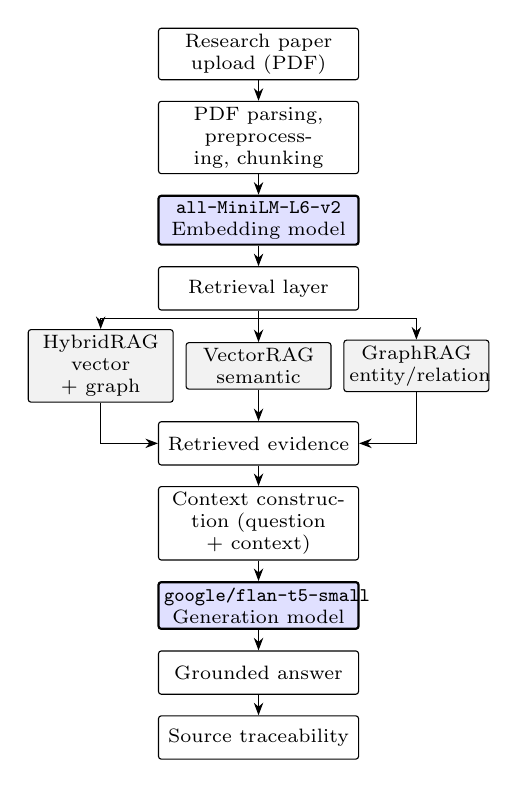
\begin{tikzpicture}[node distance=0.26cm]
\node[b](pdf){Research paper upload (PDF)};
\node[b,below=of pdf](pre){PDF parsing, preprocessing, chunking};
\node[m,below=of pre](emb){\texttt{all-MiniLM-L6-v2}\\Embedding model};
\node[b,below=of emb](ret){Retrieval layer};
\node[d,text width=1.7cm,below=0.4cm of ret](vec){VectorRAG\\semantic};
\node[d,text width=1.7cm,left=0.15cm of vec](hyb){HybridRAG\\vector + graph};
\node[d,text width=1.7cm,right=0.15cm of vec](gra){GraphRAG\\entity/relation};
\node[b,below=0.4cm of vec](ev){Retrieved evidence};
\node[b,below=of ev](ctx){Context construction (question + context)};
\node[m,below=of ctx](gen){\texttt{google/flan-t5-small}\\Generation model};
\node[b,below=of gen](ans){Grounded answer};
\node[b,below=of ans](src){Source traceability};
\draw[ar](pdf)--(pre);\draw[ar](pre)--(emb);\draw[ar](emb)--(ret);
\draw[ar](ret)--(vec);\draw[ar](ret.south)--++(0,-0.1)-|(hyb.north);
\draw[ar](ret.south)--++(0,-0.1)-|(gra.north);
\draw[ar](vec)--(ev);\draw[ar](hyb.south)|-(ev.west);\draw[ar](gra.south)|-(ev.east);
\draw[ar](ev)--(ctx);\draw[ar](ctx)--(gen);\draw[ar](gen)--(ans);\draw[ar](ans)--(src);
\end{tikzpicture}
\caption{Overall system architecture (\texttt{figures/system\_architecture}). The embedding model (\texttt{all-MiniLM-L6-v2}) feeds the retrieval layer; the generation model (\texttt{google/flan-t5-small}) produces the answer from the question and retrieved evidence.}
\label{fig:system}
\end{figure}

\subsection{Embedding Model}
\texttt{sentence-transformers/all-MiniLM-L6-v2} \cite{hf_minilm,reimers2019sbert,wang2020minilm} converts text into dense vectors. It is applied to document chunks and to user queries, which allows semantic similarity to be computed between them:
\begin{equation*}
\text{Chunk}\rightarrow\text{MiniLM}\rightarrow \mathbf{d},\qquad
\text{Query}\rightarrow\text{MiniLM}\rightarrow \mathbf{q}.
\end{equation*}
The embedding model does not generate the answer. It only supports retrieval, in particular VectorRAG. \ph{CONFIRM whether the embedding model is also used for entity or node matching in GraphRAG}.

\subsection{Generation Model}
\texttt{google/flan-t5-small} \cite{hf_flan,chung2022flan,raffel2020t5} is an instruction-finetuned encoder-decoder model. It receives the question and the retrieved context and generates the final natural-language answer:
\begin{equation*}
(\text{Question},\text{Context})\rightarrow\text{FLAN-T5-small}\rightarrow\text{Answer}.
\end{equation*}

\subsection{Model Selection}
Both models are open-source, small and suitable for local experimentation with limited resources. \texttt{all-MiniLM-L6-v2} is a compact encoder widely used for semantic retrieval, and \texttt{flan-t5-small} follows instructions and has low computational requirements. The base paper's models, \texttt{text-embedding-ada-002} and GPT-4o-mini, were not used because of accessibility, reproducibility and resource constraints \ph{CONFIRM the actual reason}. The replacement is not claimed to be superior (Fig.~\ref{fig:config}).

\begin{figure}[t]
\centering
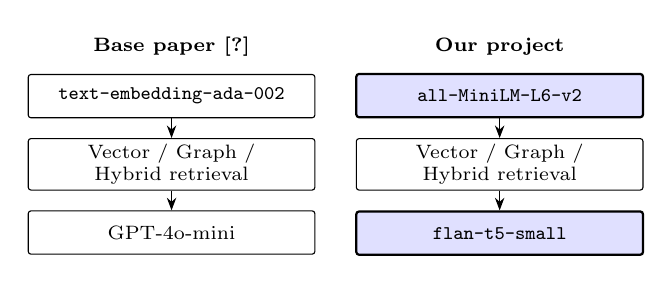
\begin{tikzpicture}[node distance=0.25cm]
\node[font=\scriptsize\bfseries](t1){Base paper \cite{ghanadian2026base}};
\node[b,text width=3.5cm,below=0.1cm of t1](a1){\texttt{text-embedding-ada-002}};
\node[b,text width=3.5cm,below=of a1](a2){Vector / Graph / Hybrid retrieval};
\node[b,text width=3.5cm,below=of a2](a3){GPT-4o-mini};
\node[font=\scriptsize\bfseries,right=0.6cm of t1,xshift=1.5cm](t2){Our project};
\node[m,text width=3.5cm,below=0.1cm of t2](b1){\texttt{all-MiniLM-L6-v2}};
\node[b,text width=3.5cm,below=of b1](b2){Vector / Graph / Hybrid retrieval};
\node[m,text width=3.5cm,below=of b2](b3){\texttt{flan-t5-small}};
\draw[ar](a1)--(a2);\draw[ar](a2)--(a3);
\draw[ar](b1)--(b2);\draw[ar](b2)--(b3);
\end{tikzpicture}
\caption{Model configuration of the base paper versus this project (\texttt{figures/config\_comparison}).}
\label{fig:config}
\end{figure}

%=====================================================================
\section{Retrieval Methodologies}
\subsection{VectorRAG}
\label{sec:vector}
Each chunk $d_i$ is embedded as $\mathbf{d}_i$ and the query as $\mathbf{q}$. Chunks are ranked by cosine similarity,
\begin{equation}
\cos(\mathbf{q},\mathbf{d})=\frac{\mathbf{q}\cdot\mathbf{d}}{\|\mathbf{q}\|\,\|\mathbf{d}\|},
\label{eq:cos}
\end{equation}
and the top-$k$ chunks form the retrieved set,
\begin{equation}
\mathcal{R}_{\text{vec}}(q)=\operatorname*{arg\,top\text{-}k}_{d_i}\ \cos(\mathbf{q},\mathbf{d}_i).
\label{eq:topk}
\end{equation}
The retrieved chunks are concatenated into a context and passed with the question to the generator (Fig.~\ref{fig:vector}). VectorRAG is effective when the query and the supporting text are semantically close, as noted in the base study \cite{ghanadian2026base}. The index is \ph{INSERT VECTOR INDEX/DATABASE} and $k=\ph{INSERT TOP-K}$.

\begin{figure}[t]
\centering
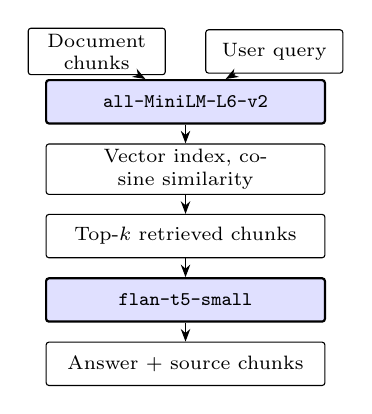
\begin{tikzpicture}[node distance=0.24cm]
\node[b,text width=1.6cm](ch){Document chunks};
\node[b,text width=1.6cm,right=0.5cm of ch](q){User query};
\node[m,text width=3.4cm,below=0.35cm of $(ch)!0.5!(q)$](e){\texttt{all-MiniLM-L6-v2}};
\node[b,text width=3.4cm,below=of e](ix){Vector index, cosine similarity};
\node[b,text width=3.4cm,below=of ix](tk){Top-$k$ retrieved chunks};
\node[m,text width=3.4cm,below=of tk](g){\texttt{flan-t5-small}};
\node[b,text width=3.4cm,below=of g](a){Answer + source chunks};
\draw[ar](ch)--(e);\draw[ar](q)--(e);
\draw[ar](e)--(ix);\draw[ar](ix)--(tk);\draw[ar](tk)--(g);\draw[ar](g)--(a);
\end{tikzpicture}
\caption{VectorRAG pipeline (\texttt{figures/vector\_rag}).}
\label{fig:vector}
\end{figure}

\subsection{GraphRAG}
\label{sec:graph}
GraphRAG represents information as a graph $G=(V,E)$ in which nodes $V$ are entities or concepts and edges $E$ are relations, for example a model that \emph{uses} a method or is \emph{evaluated on} a dataset. Construction involves entity identification, relationship extraction and graph assembly; retrieval identifies the entities in the query, locates the matching nodes and traverses neighboring nodes and edges to collect relational evidence. Unlike vector search, which scores chunks independently by similarity, graph retrieval can follow explicit links across several hops and can link information that is distributed across chunks or papers \cite{edge2024graphrag,peng2024graphragsurvey}. A retrieved node or edge is mapped back to its source chunk so that the generator receives text rather than only triples (Fig.~\ref{fig:graph}).

\ph{INSERT ACTUAL GRAPH CONSTRUCTION METHOD: entity/relation extraction tool, graph store, traversal depth, number of nodes and edges}.

\begin{figure}[t]
\centering
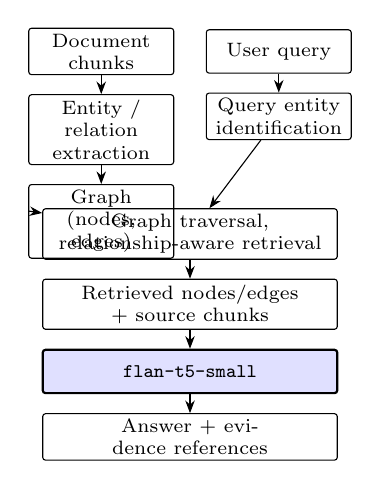
\begin{tikzpicture}[node distance=0.24cm]
\node[b,text width=1.7cm](ch){Document chunks};
\node[b,text width=1.7cm,right=0.4cm of ch](q){User query};
\node[b,text width=1.7cm,below=of ch](ex){Entity / relation extraction};
\node[b,text width=1.7cm,below=of q](qe){Query entity identification};
\node[b,text width=1.7cm,below=of ex](gs){Graph (nodes, edges)};
\node[b,text width=3.6cm,below=0.5cm of $(gs)!0.5!(qe)$](tr){Graph traversal, relationship-aware retrieval};
\node[b,text width=3.6cm,below=of tr](ev){Retrieved nodes/edges + source chunks};
\node[m,text width=3.6cm,below=of ev](g){\texttt{flan-t5-small}};
\node[b,text width=3.6cm,below=of g](a){Answer + evidence references};
\draw[ar](ch)--(ex);\draw[ar](ex)--(gs);\draw[ar](q)--(qe);
\draw[ar](gs)--(tr);\draw[ar](qe)--(tr);
\draw[ar](tr)--(ev);\draw[ar](ev)--(g);\draw[ar](g)--(a);
\end{tikzpicture}
\caption{GraphRAG pipeline (\texttt{figures/graph\_rag}).}
\label{fig:graph}
\end{figure}

\subsection{HybridRAG}
HybridRAG retrieves vector evidence $\mathcal{R}_{\text{vec}}(q)$ and graph evidence $\mathcal{R}_{\text{graph}}(q)$ and fuses them into one context,
\begin{equation}
\mathcal{C}(q)=\operatorname{Fuse}\big(\mathcal{R}_{\text{vec}}(q),\mathcal{R}_{\text{graph}}(q)\big).
\label{eq:fuse}
\end{equation}
The motivation is that vector retrieval captures semantic similarity while graph retrieval captures explicit relationships, so the two signals are complementary \cite{sarmah2024hybridrag,ghanadian2026base}. \ph{INSERT ACTUAL FUSION METHOD implemented in the project (for example union, deduplication, ordering, context budget); do not state a specific algorithm unless it is implemented}. Fig.~\ref{fig:hybrid} shows the pipeline.

\begin{figure}[t]
\centering
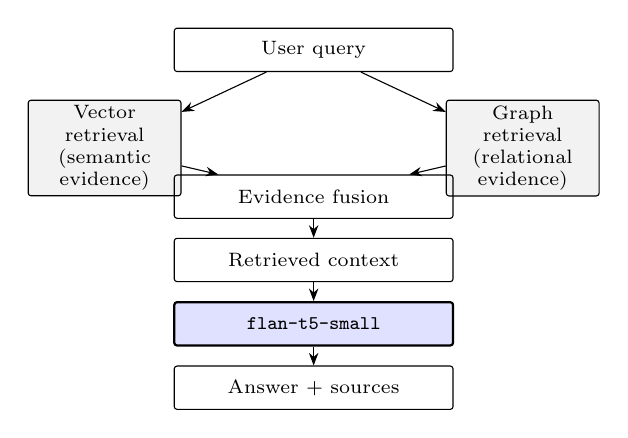
\begin{tikzpicture}[node distance=0.24cm]
\node[b,text width=3.4cm](q){User query};
\node[d,text width=1.8cm,below left=0.35cm and -0.1cm of q](v){Vector retrieval\\(semantic evidence)};
\node[d,text width=1.8cm,below right=0.35cm and -0.1cm of q](g){Graph retrieval\\(relational evidence)};
\node[b,text width=3.4cm,below=1.3cm of q](f){Evidence fusion};
\node[b,text width=3.4cm,below=of f](c){Retrieved context};
\node[m,text width=3.4cm,below=of c](t5){\texttt{flan-t5-small}};
\node[b,text width=3.4cm,below=of t5](a){Answer + sources};
\draw[ar](q)--(v);\draw[ar](q)--(g);
\draw[ar](v)--(f);\draw[ar](g)--(f);
\draw[ar](f)--(c);\draw[ar](c)--(t5);\draw[ar](t5)--(a);
\end{tikzpicture}
\caption{HybridRAG pipeline (\texttt{figures/hybrid\_rag}).}
\label{fig:hybrid}
\end{figure}

%=====================================================================
\section{Experimental Setup}
The experimental setup is described so that it can be repeated. Unless noted, all values must be taken from the actual project.
\begin{itemize}
\item \textbf{Corpus:} \ph{INSERT NUMBER OF DOCUMENTS} papers of type \ph{INSERT DOCUMENT TYPES/DOMAIN}.
\item \textbf{Scenarios:} (i) single paper, \ph{INSERT PAPER USED}; (ii) multi-paper database of \ph{INSERT NUMBER OF PAPERS} papers.
\item \textbf{Preprocessing and chunking:} \ph{INSERT PDF PARSER}; chunk size \ph{INSERT CHUNK SIZE}; overlap \ph{INSERT OVERLAP}.
\item \textbf{Models:} \texttt{sentence-transformers/all-MiniLM-L6-v2}; \texttt{google/flan-t5-small}; generation settings \ph{INSERT MAX LENGTH, DECODING}.
\item \textbf{Retrieval:} vector index \ph{INSERT INDEX}; graph representation \ph{INSERT GRAPH STORE}; top-$k$ \ph{INSERT TOP-K}.
\item \textbf{Prompt format:} \ph{INSERT PROMPT TEMPLATE}.
\item \textbf{Evaluation questions:} \ph{INSERT NUMBER OF QUESTIONS}, created by \ph{INSERT HOW QUESTIONS AND REFERENCE ANSWERS WERE OBTAINED}.
\item \textbf{Environment:} \ph{INSERT HARDWARE (CPU/GPU, RAM) AND SOFTWARE VERSIONS}.
\end{itemize}

\subsection{Evaluation Metrics}
\textbf{Cosine similarity} (Eq.~\ref{eq:cos}) is used in the base study to compare vectorized texts \cite{ghanadian2026base}. In this work it measures \ph{CONFIRM: e.g., similarity between the embedding of the generated answer and the embedding of the reference answer, and which embedding model computes it}. Because the embedding model differs between the two studies, absolute cosine values are not directly interchangeable.

\textbf{Faithfulness} measures whether the claims in a generated answer are supported by the retrieved evidence. It is important in scientific question answering because a fluent answer with unsupported claims is unreliable. The scoring procedure is \ph{INSERT FAITHFULNESS METHOD, e.g., judge model, framework such as RAGAS \cite{es2024ragas}, or manual annotation}.

No additional metrics (retrieval precision, recall, latency) are reported unless they were measured: \ph{INSERT ANY ADDITIONAL MEASURED METRICS OR DELETE THIS SENTENCE}.

%=====================================================================
\section{Results}
\subsection{Results of Our Implementation}
Table~\ref{tab:ours} reports cosine similarity and faithfulness for the three strategies in both scenarios.

\begin{table}[t]
\caption{Results of Our Implementation (\texttt{all-MiniLM-L6-v2} + \texttt{flan-t5-small})}
\label{tab:ours}
\centering
\small
\begin{tabular}{llrr}
\toprule
Scenario & RAG & Cosine Sim. & Faithfulness \\
\midrule
Single & VectorRAG & \ph{VALUE} & \ph{VALUE} \\
Single & GraphRAG  & \ph{VALUE} & \ph{VALUE} \\
Single & HybridRAG & \ph{VALUE} & \ph{VALUE} \\
Database & VectorRAG & \ph{VALUE} & \ph{VALUE} \\
Database & GraphRAG  & \ph{VALUE} & \ph{VALUE} \\
Database & HybridRAG & \ph{VALUE} & \ph{VALUE} \\
\bottomrule
\end{tabular}
\end{table}

\begin{figure}[t]
\centering
\fbox{\parbox{0.9\columnwidth}{\centering\vspace{1.2cm}\ph{PLACEHOLDER: bar chart of cosine similarity and faithfulness for VectorRAG, GraphRAG, HybridRAG in both scenarios. Generate only from the values in Table~\ref{tab:ours}.}\vspace{1.2cm}}}
\caption{Evaluation results (\texttt{figures/results.pdf}).}
\label{fig:results}
\end{figure}

\subsection{Base Paper versus Our Results}
Table~\ref{tab:baseresults} reproduces the values reported by Ghanadian et al.\ \cite{ghanadian2026base}.

\begin{table}[t]
\caption{Results Reported in the Base Paper \cite{ghanadian2026base}}
\label{tab:baseresults}
\centering
\small
\begin{tabular}{llrr}
\toprule
Scenario & RAG & Cosine Sim. & Faithfulness \\
\midrule
Single & VectorRAG & 0.670 & 0.841 \\
Single & GraphRAG  & 0.654 & 0.785 \\
Single & HybridRAG & 0.687 & 0.845 \\
Database & VectorRAG & 0.651 & 0.830 \\
Database & GraphRAG  & 0.633 & 0.761 \\
Database & HybridRAG & 0.662 & 0.834 \\
\bottomrule
\end{tabular}
\end{table}

Table~\ref{tab:compare} compares the two studies, where the difference is $\Delta=\text{ours}-\text{base}$.

\begin{table}[t]
\caption{Base Paper versus Our Results ($\Delta=\text{ours}-\text{base}$)}
\label{tab:compare}
\centering
\footnotesize
\setlength{\tabcolsep}{3pt}
\begin{tabular}{llrrrrrr}
\toprule
 & & \multicolumn{3}{c}{Cosine Sim.} & \multicolumn{3}{c}{Faithfulness} \\
\cmidrule(lr){3-5}\cmidrule(lr){6-8}
Scen. & RAG & Base & Ours & $\Delta$ & Base & Ours & $\Delta$ \\
\midrule
Single & Vector & 0.670 & \ph{V} & \ph{$\Delta$} & 0.841 & \ph{V} & \ph{$\Delta$} \\
Single & Graph  & 0.654 & \ph{V} & \ph{$\Delta$} & 0.785 & \ph{V} & \ph{$\Delta$} \\
Single & Hybrid & 0.687 & \ph{V} & \ph{$\Delta$} & 0.845 & \ph{V} & \ph{$\Delta$} \\
DB & Vector & 0.651 & \ph{V} & \ph{$\Delta$} & 0.830 & \ph{V} & \ph{$\Delta$} \\
DB & Graph  & 0.633 & \ph{V} & \ph{$\Delta$} & 0.761 & \ph{V} & \ph{$\Delta$} \\
DB & Hybrid & 0.662 & \ph{V} & \ph{$\Delta$} & 0.834 & \ph{V} & \ph{$\Delta$} \\
\bottomrule
\end{tabular}
\end{table}

\subsection{Fairness of the Comparison}
The two studies differ in the embedding model, the generation model, the corpus, chunking, graph construction, retrieval configuration, prompt design, evaluation questions and computing environment (Table~\ref{tab:config}). The comparison is intended to assess consistency and practical differences between the two implementations rather than constitute a strictly controlled reproduction of the original experimental setup. \ph{REVISE this statement if any of these conditions were in fact identical}.

\begin{table}[t]
\caption{Base Paper versus Our Implementation}
\label{tab:config}
\centering
\small
\begin{tabular}{p{1.5cm}p{2.9cm}p{2.9cm}}
\toprule
Component & Base paper \cite{ghanadian2026base} & Our project \\
\midrule
Embedding & \texttt{text-embedding-ada-002} & \texttt{all-MiniLM-L6-v2} \\
Generation & GPT-4o-mini & \texttt{flan-t5-small} \\
Retrieval & Vector/Graph/Hybrid & Vector/Graph/Hybrid \\
Dataset & Base corpus & Our corpus \ph{DESCRIBE} \\
\bottomrule
\end{tabular}
\end{table}

%=====================================================================
\section{Discussion}
VectorRAG identifies chunks that are semantically similar to the query, GraphRAG identifies explicit relations between entities and concepts, and HybridRAG supplies both semantic and relational evidence. The base study reports HybridRAG with the highest values in both scenarios, VectorRAG close behind and GraphRAG lowest on both metrics \cite{ghanadian2026base}.

\ph{INTERPRET OUR RESULTS: (1) in which scenario and on which metric VectorRAG performed well; (2) whether GraphRAG helped for relational or multi-hop questions; (3) whether HybridRAG improved on the best single strategy and by how much; (4) whether the ranking agrees with the base paper}. Observed differences from the base paper may be attributed to the smaller embedding model, the limited capacity of \texttt{flan-t5-small} to use long context and follow instructions, differences in graph construction and corpus, and different scoring procedures. These explanations are hypotheses unless tested with controlled ablations. No claim of statistical significance is made unless a test was performed: \ph{INSERT TEST OR DELETE}.

%=====================================================================
\section{Observability and Traceability}
\subsection{Observability}
Observability concerns recording what happens at each step of a query:
\begin{equation*}
\text{Query}\rightarrow\text{Retrieval}\rightarrow\text{Chunks/Nodes}\rightarrow\text{Scores}\rightarrow\text{Prompt}\rightarrow\text{Generation}\rightarrow\text{Answer}.
\end{equation*}
Useful records include the query, retrieved evidence, retrieval scores, prompt, model identifiers, response, latency and failures. Status in the present system: query \ph{IMPLEMENTED / FUTURE WORK}; retrieved evidence \ph{IMPLEMENTED / FUTURE WORK}; retrieval scores \ph{IMPLEMENTED / FUTURE WORK}; prompt \ph{IMPLEMENTED / FUTURE WORK}; latency \ph{IMPLEMENTED / FUTURE WORK}; failure logging \ph{IMPLEMENTED / FUTURE WORK}. Only capabilities marked as implemented may be reported as such.

\subsection{Source Traceability}
Traceability links an answer to its evidence:
\begin{equation*}
\text{Question}\rightarrow\text{Evidence}\rightarrow\text{Source document}\rightarrow\text{Chunk/Node}\rightarrow\text{Answer}.
\end{equation*}
It supports user trust, debugging, hallucination analysis, reproducibility and scientific verification, since a user can check a statement against the cited passage. Traceability does not guarantee that the generated statement is correct; it makes verification possible. \ph{DESCRIBE how source references are actually displayed in the system}.

%=====================================================================
\section{Limitations}
The limitations that apply to this study are as follows; \ph{EDIT to match the actual project}. The model configuration differs from the base paper, so differences cannot be attributed to a single factor. The evaluation corpus and question set are relatively small. \texttt{flan-t5-small} has limited capacity and a restricted input length, which can cause generation errors even when retrieval succeeds. Answer quality depends on retrieval quality, and graph construction is complex and error-prone. Human evaluation was limited \ph{CONFIRM}, and the metrics used are approximations of answer quality.

\section{Technical Contributions and Course Learning}
\textbf{Research:} evaluation of retrieval strategies under an open-source lightweight configuration. \textbf{Engineering:} an end-to-end literature assistant. \textbf{Experimental:} comparison with the findings of the base paper. \textbf{Practical:} source traceability and, where implemented, observability.

Table~\ref{tab:modules} relates the project to the course modules and distinguishes directly applied from conceptually learned material.

\begin{table}[t]
\caption{Mapping to Course Modules}
\label{tab:modules}
\centering
\footnotesize
\begin{tabular}{p{3.9cm}p{1.1cm}p{2.0cm}}
\toprule
Module & Status & Relevance \\
\midrule
1 Language and NLP foundations & Applied & Text preprocessing \\
2 Statistical language models & Conceptual & Background \\
3 Neural networks and embeddings & Applied & Embeddings \\
4 Neural LMs and sequence models & Conceptual & Seq2seq generation \\
5 Transformer architecture & Applied & MiniLM, T5 \\
6 LLM training, foundation models & Conceptual & Background \\
7 Fine-tuning and adaptation & Conceptual & No fine-tuning \ph{CONFIRM} \\
8 Efficient LLMs & Applied & Small models \\
9 Advanced and responsible LLMs & Applied & RAG, grounding \\
\bottomrule
\end{tabular}
\end{table}

%=====================================================================
\section{Conclusion and Future Work}
This paper implemented VectorRAG, GraphRAG and HybridRAG for scientific literature question answering using \texttt{all-MiniLM-L6-v2} for semantic representation and \texttt{flan-t5-small} for generation, and compared the strategies with the findings of a base study that used \texttt{text-embedding-ada-002} and GPT-4o-mini \cite{ghanadian2026base}. The evaluation used cosine similarity and faithfulness in single-paper and multi-paper scenarios, and the main finding is \ph{INSERT KEY FINDING}. The results indicate how retrieval strategy and model selection influence answer quality, and the study illustrates how grounded generation with source traceability can support more reliable literature exploration.

Future work includes stronger embedding and open-source generation models, reranking, adaptive retrieval, improved graph construction and fusion, citation verification, human evaluation, larger benchmarks, table and figure understanding, scalable multi-document retrieval, improved observability and production deployment.

\bibliographystyle{IEEEtran}
\bibliography{references}

\end{document}
